%\UseRawInputEncoding
\documentclass[class=article,crop=false]{standalone}
\usepackage{../pacco}
\begin{document}
	\section{Continuous time Markov chains}
	\begin{definition}
		A \enf{continuous time Markov chain (CTMC)} is a stochastic process $\{X(t), t \in T\}$ with index set $T=[0,+ \infty)$ taking values in a countable set $S$, s.t. 
		\begin{equation*}
			\mathbb{P}(X(t_n)=i_n | X(t_0)=i_0, \dots, X(t_{n-1})= x(t_{n-1}))
		\end{equation*}
		i.e. the Markov property holds for all $i_0, \dots, i_n \in S$ and $0\leqslant t_0 < \dots < t_n$. \\
		We can define the transition probability 
		\begin{equation*}
			p_{ij}(s,s+t):= \mathbb{P}(X(s+t)=j|X(s)=i)
		\end{equation*}
		for $t>0$, which we assume are time homogeneoCus, i.e. depend on $t$ not on $s$. Hence we can define 
		\begin{equation*}
			p_{ij}(t):= p_{ij}(0,t)
		\end{equation*}
		since $p_{ij}(s,s+t)= p_{ij}(0,t)$.\\
		Set \[p_{ij}(0):=\delta_{ij}=\begin{cases}
			1 &i=j\\
			0 &i\neq j.
		\end{cases}\]
	\end{definition}
	\begin{example}
		The Poisson process with intensity $\lambda>0 $ is defined by $X(0)=0$ a.s. and 
		\begin{equation*}
			p_{ij}(t)= \frac{(\lambda t)^{j-1}e^{-\lambda t}}{(j-i)!}, \hspace{0.5 cm} j \geqslant 1
		\end{equation*}
		and $0$ elsewhere. We see it is time-homogeneous on $S = \mathbb{Z}_+$. The increments are s.t.
		\begin{equation*}
			X(s+t)-X(s) \sim Poisson (\lambda t)
		\end{equation*}
		and if we set $s=0$, then $X(t) \sim Poisson(\lambda t)$.
	\end{example}
	\begin{exercise}
		Show that the transition function of a MTMC, together with an initial distribution, determines all joint distribution 
		\begin{equation*}
			\mathbb{P}( X(t_0)=i_0, \dots, X(t_{n})= x(t_{n}))
		\end{equation*}
		for all choice of $i_0, \dots, i_n$ and $t_o <\dots < t_n$. \\
	\end{exercise}
	Denote $P_t$ the square matrix with entries $\{p_{ij}(t)\_{i, j \in S}$. \\
	the family of $\{P_t\}_{t\geqslant 0}$ is called \enf{transition semigroup}, since:
	\begin{itemize}
		\item $\sum_{j \in S} p_{ij} = 1$: row sum
		\item $P_0=I$ (i.e. $p_{ij}(0):=\delta_{ij}$)
		\item $P_{t+s}= P_t P_s$:  \enf{semigroup property}, namely the Chapman-Kolmogorov's equations 
		\begin{equation*}
			p_{ij}(s+t)= \sum_{k \in S} p_{ik}(s) p_{kj}(t)
		\end{equation*}
	\end{itemize}
	We will assume $P_t$ is continuous at the origin (called \textit{standard})
	\begin{equation*}
		p_{ij}(t) \rightarrow \delta_{ij} \hspace{0.5 cm} t \rightarrow 0
	\end{equation*}
	which implies continuity at all $t>0$.\\
	$P_t$ is parametrized by time, and ideally we would like on object similar to the transition matrix for DTMC's, , relative to the temporal unit. We look at infinitesimal intervals. 
	\begin{definition}
		The matrix $Q$ given by 
		\begin{equation*}
			Q= \frac{d}{dt}P_t |_{t=0}
		\end{equation*}
		is called infinitesimal generator of the chain, and its entries $(q_{ij})_{i,j \in S}$ are called \enf{infinitesimal rates}.
	\end{definition}
	\begin{proposition}
		Let $P_t$ be a continuous transition semigroup on $S$ countable. For all $i,j$ the quantity $q_{ij}:=p'_{ij}(0)$ exists and 
		\[q_{ij} \in
		\begin{cases}
			[0,\infty) & j \neq i \\
			[-\infty, 0] & j = i \\
		\end{cases}
		\]
		For $j \neq i$
		\begin{equation*}
			q_[ij] = \lim_{h \rightarrow 0} \frac{p_{ij}(h) - \overbrace{p_{ij}(0)}^{0}}{h}
		\end{equation*}
		%In a small time interval there is a  negligibile probability that the chain goes to (?infinity)
	\end{proposition}
	\begin{itemize}
		\item  $\implies p_{ij}(h)=q_{ij}h + o(h)$ 
		\item  $\implies X$ goes to $j$ from $i$ with probability approximately $q_{ij}h $.
		\item  $\implies o(h)$ collects the error of approximation and all other events (for example, $X$) goes to $k$ before $j$).
	\end{itemize}
	So the chain has at most one jump at each instant. When $j=i$, since $p_{ii}(0) = 1$, the above calculation gives $q_{ii} \leqslant 0$. \\
	Sometimes we will denote $q_i = - q_{ii}$.
	\begin{definition}
		A state $i$ is called
		\begin{itemize}
			\item \enf{absorbing} if $q_i = 0$
			\item \enf{stable} if $0 < q_i < \infty$
			\item \enf{instantaneous} if $q_i = \infty$ 
		\end{itemize}
		If $\sup_{i \in S} q_i < \infty, Q$ is \textbf{stable}. \\
		If $q_i = \sum_{j \neq i} q_{ij}, \hspace{0.2 cm} \forall i \in S, Q $ is called \enf{conservative}.     
	\end{definition}
	\begin{remark}
		The absolute value of the diagonal entry equals the sum of the off-diagonal entries.
	\end{remark}\begin{equation*}
		1 = \sum_{j \in S} p_{ij}(h) = \sum_{j \neq i} p_{ij}(h) + p_{ii}(h)
	\end{equation*}
	which leads to 
	\begin{equation*}
		\frac{1-p_{ii}(h)}{h} = \sum_{j \neq i} \frac{p_{ij}(h)}{h}
	\end{equation*}
	Taking the limit as $h$ decreases to $0$, we get
	\begin{equation*}
		q_i = \lim_{h \downarrow 0} \sum_{j \neq i} \frac{p_{ij}(h)}{h}
	\end{equation*}
	If limit and sum exchange, we get 
	\begin{equation*}
		q_i = \sum_{j \neq i} q_{ij} \implies \sum_{j \in S} q_{ij} = 0
	\end{equation*}
	\begin{remark}
		Conservativity comes from the fact that transition probabilities conserve the mass.
	\end{remark}
	We assumed we had the transition probabilities are available but this is rarely the case. In many cases, when we move on to general and complex spaces, probabilities are specified through the generator (instead of the transition semigroup).
	We are going to argument later that this gives complete information about the process too, but if we have the generator, how can we check that the implied process is well defined? We need criteria to be checked on the generator. Often, only $Q$ is available, while $P_t$ is unknown. So, this identity relates to the conservation of probability mass by the transition semigroup. So it is enough to check that $Q$ row sums are null (to verify this condition). \\
	If $Q$ is stable and conservative, $q_i$ is interpreted as the rate of leaving the state $i$. So
	\begin{equation*}
		p_{ii}(h) = 1-q_i h + o(h) 
	\end{equation*}
	If 
	\begin{itemize}
		\item $q_i = 0$, then $X$ leaves $i$ at rate $0$, so $i$ is absorbing. 
		\item $q_i = \infty$, then $x$ leaves the state $i$ instantaneously. 
	\end{itemize}
	\begin{proposition}
		A CTMC with finite state space is always stable and conservative.
	\end{proposition}
	So we can reverse the statement, saying that trouble scenario happen when the chain is not stable or not  conservative.
	\begin{example}
		Consider $X$ on $\mathbb{Z}_+$ with 
		\begin{equation*}
			q_{i,i+1}= \lambda \hspace{0.5 cm} q_{i,i-1}= i \hspace{0.5 cm} q_{ii}= -(\lambda + i)
		\end{equation*}
		and $0$ elsewhere. $Q$ is conservative ($P_t$ would be well defined, if we knew it) but 
		\begin{equation*}
			\sup_{i \in S} q_i = \sup_{i \geqslant 0} \lambda + i = \infty
		\end{equation*}
		so it is not stable. \\
		The meaning of this distinction will be treated later.
	\end{example}
	\begin{definition}
		A general class of stable and conservative CTMC's is given by \textbf{regular jump processes} such that 
		\begin{itemize}
			\item their paths are piecewise constant: for almost all $\omega$ and all $t \geqslant 0, \exists \varepsilon = \varepsilon(t,\omega)$ such that 
			\begin{equation*}
				X(t+s,\omega) = X(t,\omega) \hspace{0.5 cm} \forall s \in [0,\varepsilon]
			\end{equation*}
			This means that the chain remains where it is for a positive amount of time. 
			\item they have finitely many points of discontinuity in every bounded time interval.
		\end{itemize}
	\end{definition}
	The typical behaviour is the one represented in Figure \ref{regjump}. %metti figura. sì capo \\
	For example, \textbf{explosive chains} are not regular in the above sense (see Figure \ref{xplchain}): these chains have closer and closer jumps until there are infinitely many around $x=s$.%metti altra figura). fatto capo\\
	
	\begin{minipage}{0.5\textwidth}
		\begin{figure}[H]
			\centering
			\includegraphics[scale=0.6]{../standalones/pdfs/regjump}
			\caption{Regualar jumps process}
			\label{regjump}
		\end{figure}
	\end{minipage} \hfill
	\begin{minipage}{0.45\textwidth}
		\begin{figure}[H]
			\centering
			\includegraphics[scale=0.6]{../standalones/pdfs/xplosive}
			\caption{explosive chain}
			\label{xplchain}
		\end{figure}
	\end{minipage}
	
	\begin{example}
		\enf{Poisson process}
		\begin{align*}
			&p_{ij}(t)=\frac{(\lambda t)^{j-i}e^{-\lambda t}}{(j-i)!}\qquad j\geqslant 1\\
			\implies &p_{ii}(t)=e^{-\lambda t}\\
			&p_{i,i+1}(t)=\lambda t e^{-\lambda t}\\
			&p_{i,i+k}(t)=\frac{(\lambda t)^{k}e^{-\lambda t}}{k!}\\
			\implies &q_{ii}=-\lambda,\quad q_{i,i+1}=\lambda,\qquad\text{and 0 elsewhere.}
		\end{align*}
		\textit{Interarrival times}: $T_i$ waiting time in $i$.
		\begin{align*}
			\mathbb{P}(T_0 > t) &= \mathbb{P}(X(t) = 0|X(0) = 0) = e^{- \lambda t}\\
			\implies \mathbb{P}(T_0 < t) &= 1-e^{-\lambda t} \implies T_0 \sim \text{Exp}(\lambda)
		\end{align*}
		So $\prob(T_i>t|T_0=t_0,\ldots,T_{i-1}=t_{i-1})=$
		\begin{align*}
			s &= t_0+\ldots+t_{i-1}\\
			&=\prob(x(s+t)=i|x(s)=i)=e^{-\lambda t}\\
			&\implies T_i\sim\text{Exp}(\lambda)
		\end{align*}
	\end{example}
	\begin{example}(Birth and Death processes)\\
		Denote B\&D$(\lambda _i, \mu_i)$ such that 
		\[q_{ij} = 
		\begin{cases}
			\lambda_i & j = i+1  \hspace{0.5 cm} i \geqslant 0 \\
			\mu_i  & j = i-1  \hspace{0.5 cm} i > 0 \\
			0 & \text{elsewhere} \\
		\end{cases}
		\]
		\begin{equation*}
			q_{ii} = - (\lambda _ i + \mu_i)
		\end{equation*}
		%figura arriva!!
		\begin{figure}[H]
			\centering
			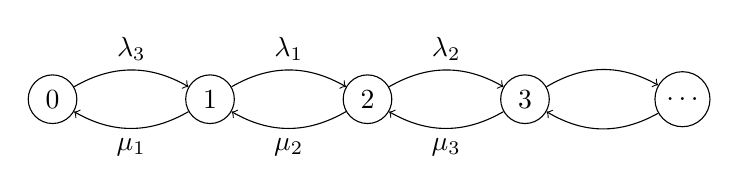
\begin{tikzpicture}[->,node distance=2cm]
				\node[circle,draw](zero){0};
				\node [circle,draw] (one) [right of=zero] {1};
				\node [circle,draw] (two) [right of=one] {2};
				\node [circle,draw] (three) [right of=two] {3};    
				\node [circle,draw] (dots) [right of=three]{$\ldots$};
				\path (one) edge [bend left] node [above] {$\lambda_1$} (two);
				\path (two) edge [bend left] node [above] {$\lambda_2$} (three);
				\path (three) edge [bend left] node [below] {$\mu_3$} (two);
				\path (two) edge [bend left] node [below] {$\mu_2$} (one);
				\path (three) edge [bend left] node [below] {} (dots);
				\path (dots) edge [bend left] node [below] {} (three);
				\path (zero) edge [bend left] node [above] {$\lambda_3$} (one);
				\path (one) edge [bend left] node [below] {$\mu_1$} (zero);
			\end{tikzpicture}
			\label{bedcontinuous}
		\end{figure} whose invariant $\pi$ is the uniform on on $S_0$. Let $\tau$ be a finite random time on $\N$, independent of $Y$, such that:  
	\end{example}
	Special cases:
	\begin{itemize}
		\item $\mu_i=0 \;\forall i, \lambda_i > 0$ \textbf{Birth process} which can be 
		\begin{itemize}
			\item [$\star$] Poisson
			\item [$\star$] $\lambda_i = \underbrace{\lambda}_{\mathclap{\text{per capita birth rate}}}\cdot i $ (\enf{Yule process})
		\end{itemize}
		$\lambda_i = \lambda \cdot i + c$, adding immigration rate $c$.
		\item $\lambda_i = 0 \forall i, \mu_i > 0$ (\enf{Pure death process})
	\end{itemize}
	For example, if 
	\begin{equation*}
		\lambda_i = \lambda \cdot i, \hspace{0.5 cm} \mu_i = \mu \cdot i
	\end{equation*}
	the transition probabilities are very complicated to find, like in the following case: the process has $i = 1$
	\begin{equation*}
		p_{1j}(t) = (1-\mu \gamma) (1-\lambda \gamma) (\lambda \gamma)^{j-i}
	\end{equation*}
	where 
	\begin{equation*}
		\gamma= \frac{e^{(\lambda-\mu) t} - 1}{\lambda e^{(\lambda - \mu)t}-\mu}
	\end{equation*}
	If $X$ is specified only through the generator $Q$, a general task is to be able to describe the transition semigroup (which is difficult in general). \\
	A first tool to do so is given by the so called \textbf{Kolmogorov's equations}.
	\begin{theorem}
		Let $Q$ be stable and conservative. Then, $P_t$ and $Q$ satisfy:
		\begin{itemize}
			\item The \enf{backward equation}
			\begin{equation*}
				P'_t =  Q P_t \hspace{1 cm} p'_{ij}(t) = \sum_{k \in S} q_{ik}p_{kj}(t)
			\end{equation*}
			\item If 
			\begin{equation*}
				\sum_{k \in S} p_{ik}(t) q_k < \infty
			\end{equation*}
			the \enf{forward equation}
			\begin{equation*}
				P'_t = P_t Q \hspace{1 cm} p'_{ij}(t) = \sum_{k \in S} p_{ik}(t)q_{kj}
			\end{equation*}
		\end{itemize}
	\end{theorem}
	\begin{exercise}
		Prove the forward equation for $S$ finite using CK and linearization.\\
		The intuition consists in thinking about the backwards equation.
		\begin{figure}[H]
			\centering
			    \begin{tikzpicture}[-,>=stealth', line width=0.5pt, node distance=0.5cm]

        \node [circle, draw,  fill, label=left:$i$] (two) []{};

        \node [circle, draw,  fill] (c) [right=1cm of two]{};
        \node [circle, draw,  fill] (b) [above of=c] {};
        \node [circle, draw,  fill] (a) [above of= b]{};
        
        
        \node [circle, draw,  fill] (d) [below of=c]{};
        \node [circle, draw,  fill] (e) [below of=d]{};
        

        \node [circle, draw, fill, label=right:$j$,  circle] (j) [right= 1 cm of c]{};

        \path (two) edge node [below] {} (a);
        \path (two) edge node [below] {} (b);
        \path (two) edge node [below] {} (c);
        \path (two) edge node [below] {} (d);
        \path (two) edge node [below] {} (e);

        \path (a) edge node [below] {} (j);
        \path (b) edge node [below] {} (j);
        \path (c) edge node [below] {} (j);
        \path (d) edge node [below] {} (j);
        \path (e) edge node [below] {} (j);

        \node[circle][above right=12pt and 6pt of two]{$h$};
         \node[circle][above left=12pt and 6pt of j]{$t$};
    \end{tikzpicture}
		\end{figure}
		To obtain an intuition for the forward equation, let the second interval go to $0$.\\
		\\
		In principle (which boils down to simple cases), one could solve the Kolmogorov's equations to find the semigroup. \\
	\end{exercise}
	\begin{exercise}
		Consider the generator of the Poisson process:
		\begin{equation*}
			q_{i,i+1}=\lambda \hspace{1 cm} q_{ii} = - \lambda
		\end{equation*}
		Derive the transition probabilities from Kolmogorov's equations.  
	\end{exercise}
	First of all, we are going to analyze an example to show how Kolmogorov equations can be used and also their complexity. Let's recall the Kolmogorov Backward Equation
	\begin{equation*}
		p'_{ij}(t) = \sum_{k \in S} q_{ik}p_{kj}(t)
	\end{equation*}
	and the Kolmogorov Forward Equation
	\begin{equation*}
		p'_{ij}(t) = \sum_{k \in S} p_{ik}(t) q_{kj}
	\end{equation*}
	which provide a relationship between $P_t$ and $Q$. In simple cases they can be solved. 
	\begin{example}\enf{Poisson Process}
		\begin{equation*}
			q_{i,i+1} = \lambda \hspace{1 cm} q_{ii} = -\lambda \text{ and } 0 \text{ elsewhere}
		\end{equation*}
		Let's consider the K.F.E. and let's consider 
		\begin{itemize}
			\item $j=i$:
			\begin{equation*}
				p'_{ii}(t) = p_{ii}(t) q_{ii} = -\lambda p_{ii}(t)
			\end{equation*}
			$k = i$ necessarily. This yields
			\[
			\begin{cases}
				p_{ii}(t) & = c e ^{-\lambda t} \\
				p_{ii}(0) & = 1 \implies c = 1 \\ 
			\end{cases}
			\]
			We find the constant using the boundary condition $p_{ii}(0) = 1 $.
			\item $j > i$
			\begin{figure}[H]
				\centering
				\documentclass{standalone}			
\usepackage{../pacco}	
\begin{document}
\begin{tikzpicture}[-,>=stealth', line width=0.5pt, node distance=0.5cm]
	
	\node [circle, draw,  label=left:$i$] (two) []{};
	\node [circle, draw] (tre) [above of=two] {};
	\node [circle, draw] (quattro) [above of=tre] {};
	\node [circle, draw] (cinque) [above of=quattro] {};
	
	\node [circle, draw] (c) [right=3cm of two]{};
	\node [circle, draw] (b) [above of=c] {};
	\node [circle, draw] (a) [above of= b]{};
	
	
	\node [circle, draw] (d) [above of=a]{};
	\node [circle] (e) [above of=d]{$t^-$};
	
	
	\node [circle, draw, label=right:$j$,  circle] (j) [right= 1 cm of d]{};
	\node [circle,draw](ciao)[below of=j]{};
	\node [circle,draw](come)[below of=ciao]{};
	\node [circle,draw](stai)[below of=come]{};
	\node [circle](MALE)[above of=j]{$t$};
	
	\path (two) edge [->]node [below] {} (a);
	\path (two) edge [->]node [below] {} (d);
	\path (a) edge [->]node [below] {} (j);
	\path (d) edge [->]node [below] {} (j);
\end{tikzpicture}
\end{document}

			\end{figure}
				\begin{align*}
				p'_{ij}(t) &= p_{i,j-1}(t) q_{j-1,j} + p_{ij}(t) q_{jj}\\
				&= \lambda p_{i,j-1}(t) - \lambda p_{ij}(t)
			\end{align*}
			Now, multiply by $e^{\lambda t}$ and get from
			\begin{equation*}
				p'_{ij}(t) = \lambda p_{i,j-1}(t) - \lambda p_{ij}(t) 
			\end{equation*}
			the following
			\begin{equation*}
				\underbracket{e^{\lambda t} p'_{ij}(t) + \lambda e^{\lambda t}}_{\frac{\dif}{\dif t}\left\{e^{\lambda t}p_{ij}(t)\right\}}=\lambda e^{\lambda t}p_{i,j-1}(t)
			\end{equation*}
			%manca un pezzo
			
			assume $p_{i,j-1}(t) = \frac{(\lambda t)^{j-i-1}e^{-\lambda t}}{(j-i-1)!}$
			and integrate to get
			\begin{equation*}
				\frac{d}{dt}(e^{\lambda t} p_{ij}(t)) = \lambda \cancel{e^{\lambda t}} \frac{(\lambda t)^{j-i-1}\cancel{e^{-\lambda t}}}{(j-i-1)!} = \frac{\lambda^{j-i}}{(j-i-1)!} t ^{j-i-1}
			\end{equation*}
			Which leads to 
			\begin{equation*}
				e^{\lambda t}p _{ij}(t) =  \frac{\lambda^{j-i}}{(j-i-1)!} \frac{t ^{j-i-1} }{j-i} + c'
			\end{equation*}      
			which yields
			\[
			\begin{cases}
				p_{ij}(t) &= \frac{(\lambda t)^{j-i}e^{-\lambda t}}{(j-i)! } + c' \\
				p_{ij}(0) = 0 \implies c' = 0
			\end{cases}
			\]
			\end{itemize}
	\end{example}
What are the general solutions of the Kolmogorov equations?
\begin{theorem}
	Let $S$ be finite. Then
	\begin{equation*}
		P_t = e^{tQ}, \hspace{1 cm} P_0 = I
	\end{equation*}
	is a stochastic semigroup and the unique solution of the K.E.'s. 
\end{theorem}
\begin{remark}
		The matrix exponential
	\begin{equation*}
		e^{tQ}:= \sum_{n \geqslant 0} \frac{(tQ)^n}{n!} 
	\end{equation*}
	is convergent component-wise since $e^{t q_{ij}} < \infty, \forall t > 0$. 
\end{remark}
If $A,B$ commute, 
\begin{equation*}
	e^{A+B} = e^A e ^B
\end{equation*}
which yields
\begin{equation*}
	P_{t+s} = e^{t+s}Q = e^{tQ} e^{sQ} = P_t P_s
\end{equation*}
Intuition: consider 
\begin{equation*}
	\begin{split}
		p_{ij}(t)&= \delta_{ij}+q_{ij}t+ o(t) \hspace{0.5cm}\forall i,j\\
		P_t&=I+tQ+ o(t)
	\end{split}
\end{equation*}
Use the semigroup property to split $[0,t]$ into $n$ subintervals, so 
\begin{equation*}
	P_t= \underbrace{P_{\frac{t}{n}} \dots P_{\frac{t}{n}}}_{n \text{ times }} = (I+tQ+ o(t))^n
\end{equation*}
which generate the exponential $e^{tQ}$ as $n \rightarrow + \infty$. The generator also gives important information about the trajectories of the chain. \\
\begin{definition}
		Define the Holding Times (or waiting).
	\begin{equation*}
		T_i = \inf\{t \geqslant 0: X(s+t)\neq i | X(s)=i\}
	\end{equation*}
	in state $i\in S$, with $T_i=\infty$ if $i$ absorbing.
\end{definition}
\begin{proposition}
		Let $X$ be a regular jump CTCM with generator $Q$, and let $T_i$ be the first holding time given $X(0)=i$. Then\begin{itemize}
		\item $T_i \sim Exp(q_i)$
		\item for $j \neq i$
		\begin{equation*}
			\mathbb{P}(X(T_i)=j|X(0)=i) = \frac{q_{ij}}{q_i}
		\end{equation*}
		and these are independent. 
	\end{itemize}
\end{proposition}
Interpretation:
\begin{figure}[H]
	\centering
	\begin{tikzpicture}%[scale=0.8]
\begin{axis}[
                xlabel=\empty,
                x axis line style={->,opacity=100},
                ylabel=\empty,
                xmin=-1, xmax=100,
                ymin=-1, ymax=100,
                axis y line=left,
                y axis line style={->,opacity=100},
                ytick={20,60,40},
                yticklabels={$h$,$j$,$i$},
                xtick=\empty,
                axis x line*=bottom
                        ]
                        \draw [dashed, thick] (0,20)--(95,20) node[RedViolet,circle,midway,inner sep=2pt,yshift=10pt]{Exp($q_{ih}$)};
                        \draw [dashed, thick](0,60)--(95,60) node[RedViolet,circle,midway,inner sep=2pt,yshift=10pt]{Exp($q_{ij}$)};
                        \draw [dashed, thick](0,40)--(95,40);

\end{axis}
\end{tikzpicture}
\end{figure}
We can immagine that at every state there is a poisson process that rings at every time, exponential (?????).\\
There is a Poisson prosses with rate $q_{ij}$ each $j \neq i$ acting as a clock (all independent). Competing clocks: the first ringing sets the new state.\clock[0.1]{10}{3}{6} \\
We know 
\begin{equation*}
	\begin{split}
		Z_k &\stackrel{ind}{\sim} Exp (\lambda_k)\\
		&\implies  \min_k Z_k \sim Exp (\sum_k \lambda_k) \hspace{0.5 cm} \text{ shortest interval}\\
		&\mathbb{P}(\min_{k\neq i} Z_k=Z_j)= \frac{\lambda_j}{\sum_h \lambda_h} hspace{0.5 cm} \text{ prop of j-th is the fist to ring}
	\end{split}
\end{equation*}
So $T_i \sim Exp(\sum_{j\neq i}q_{ij})= Exp(q_i)$ and given $T_i$, the probability of going to $j$ is 
\begin{equation*}
	\frac{q_{ij}}{\sum_{j\neq i}q_{ij}}= \frac{q_{ij}}{q_i}
\end{equation*}
We can extend the above to the entire trajectory of the CTMC through the strong Markov property:
\begin{theorem}
	A regular jump CTMC $X$ with generator $Q$ is a strong markov process, i.e. 
	if $\tau$ is a stopping time w.r.t. to $\mathcal{F}_t ^X= \sigma(X_u, u \leqslant t)$, 
	conditional on $\tau <\infty$ and $X(\tau)=i$, $\{X(\tau+t), t\geqslant 0\}$ is a CTMC with initial distribution $\delta_i$ and generato $Q$, independent of $\{X(u), u\leqslant t\}$
\end{theorem}
If we now denote 
\begin{itemize}
	\item $T^{(1)}, T^{(2)}, \dots$ successive holding times 
	\item  $S_n= \sum_{i=1}^n T^{(i)}$ jumps times (Stopping times)
	\item $X_n:= X(S_n)$
\end{itemize}
\begin{figure}[H]
	\centering
	\begin{tikzpicture}%[scale=0.8]
\begin{axis}[
                xlabel=\empty,
                x axis line style={->,opacity=100},
                ylabel=\empty,
                xmin=-1, xmax=100,
                ymin=-1, ymax=100,
                axis y line=left,
                y axis line style={->,opacity=100},
                ytick={20,60,40},
                yticklabels={$X_0$,$X(S_1)=X_1$,$X(S_2)=X_2$},
                xtick={30,60},
                xticklabels={$S_1$,$S_2$},
                axis x line*=bottom
                        ]
                        \draw (0,20)--(30,20) node[circle,fill=RedViolet, pos=0,inner sep=2pt]{};
                        \draw (30,60)--(60,60) node[circle,fill=RedViolet, pos=0,inner sep=2pt]{};
                        \draw (60,40)--(95,40) node[circle,fill=RedViolet, pos=0,inner sep=2pt]{};
                        \draw[dashed] (30,20)--(30,0);
                        \draw[dashed] (60,60)--(60,0);
                        \draw[dotted,thin] (0,40)--(60,40);
                        \draw[dotted,thin] (0,60)--(30,60);
\end{axis}
\node[RedViolet,below right=0.1cm and 0.43cm, font=\footnotesize] (T) {Exp$(q_{x_0})$};
\node[RedViolet,below right=0.1cm and 2.55cm, font=\footnotesize] (Te) {Exp$(q_{x_1})$};
\node[above right=0.0cm and 0.63cm, font=\footnotesize] (T) {$T^{(1)}$};
\node[above right=0.0cm and 2.75cm, font=\footnotesize] (Te) {$T^{(2)}$};
\end{tikzpicture} 
\end{figure}
$X_n$ is  a DTMC called \textbf{embedded chain} with transition probabilities 
\begin{equation*}
	p_{ij}= \begin{cases}
		\frac{q_{ij}}{q_i} \hspace{0.5cm}&j \neq i \\
		0 &j =i
	\end{cases}
\end{equation*}
Note $X_n$ is not allowed self transitions. Given $(X_n)_{n \geqslant 1}$
\begin{equation*}
	T^{(n)}\stackrel{\text{ind}}{\sim} Exp(q_{X_{n-1}})
\end{equation*}
We have factorised the state set of the chain.
\begin{example}
	\enf{Birth and Death $(\lambda _i, \mu_i)$}:
	\[q_{ij} = 
	\begin{cases}
		\lambda_i & j = i+1, i \geqslant 0 \\
		\mu_i & j= i-1, i > 0\\
		0 &\text{ elsewhere}
	\end{cases}
	\]
	\begin{equation}
		q_{ii} = - (\lambda _i + \mu_i), \hspace {0.5 cm} q_i = \lambda _ i + \mu_i
	\end{equation}
	$\implies$ holding times in $i$ are 
	\begin{equation*}
		T_i \sim \text{ Exp} (q_i) = \text{ Exp }(\lambda_i + \mu_i)
	\end{equation*}
	$\implies$ embedded chain $X_n$ has transitions 
	\[p_{ij}
	\begin{cases}
		\frac{\lambda_i}{ \lambda _ i + \mu_i} & j = i+1 \\
		\frac{\mu_i}{ \lambda _ i + \mu_i} & j = i-1 \\
		0 & \text{ elsewhere}
	\end{cases}
	\]
\end{example}
A corollary of the above argument is the following:
\begin{proposition}
	Two regular jump CTMC's woth the same $Q$, and initial distributions, have the same transition semigroup.
\end{proposition}
This is important since we know we can proceed even without the semigroup. Embedded chain and holding times are fully determined by th egenerator $Q$, which therefore provides an equivalent characterization of the CTMC. The above suggests an imemdiate strategy to simulate the chain's trajectory:
\begin{itemize}
	\item Draw $X_0$ from the initial distribution
	\item for $n \geqslant 1, $if $X_{n-1} = i$
	\begin{itemize}
		\item [-] draw $T \sim \text{Exp}(q_i)$
		\item [-] given $T = t$, set
		\begin{equation*}
			X(t) = j \text{ with probability } \frac{q_{ij}}{q_i}
		\end{equation*}
		called \textbf{gillespie} algorithm.
	\end{itemize}
\end{itemize}
So, given a CTMC and generator - for every state - we draw the exponential with parameter represented by the first state and then we draw the normalized probabilities, iterating this process.\\
Another subclass of CTMC which allows for an explicit description of $P_t$ is the one defined below.
\begin{definition}
	Let $Y_n$ be a CTMC with transition matrix $\hat{P}$, and $N(t)$ a Poisson process with rate $\lambda$, independent of $Y_n$. The process
	\begin{equation*}
		X(t) := Y_{N(t)}   
	\end{equation*}
	is called \textbf{uniform chain with jump matrix} $\hat{P}$.         
\end{definition}
\begin{figure}[H]
	\centering
	\begin{tikzpicture}%[scale=0.8]
\begin{axis}[
                xlabel=\empty,
                x axis line style={->,opacity=100},
                ylabel=\empty,
                xmin=-1, xmax=100,
                ymin=-1, ymax=100,
                axis y line=left,
                y axis line style={->,opacity=100},
                ytick={20,60,40},
                yticklabels={$Y_0$,$Y_1$,$Y_2=Y_3$},
                xtick=\empty,
                axis x line*=bottom
                        ]
                        \draw (0,20)--(30,20) node[circle,fill=RedViolet, pos=0,inner sep=2pt]{};
                        \draw (30,60)--(50,60) node[circle,fill=RedViolet, pos=0,inner sep=2pt]{};
                        \draw (50,40)--(85,40) node[circle,fill=RedViolet, pos=0,inner sep=2pt]{};
                        \draw (85,40)--(100,40) node[circle,fill=RedViolet, pos=0,inner sep=2pt,label={self-transition}]{};
                        \draw[dashed] (30,20)--(30,0);
                        \draw[dashed] (50,60)--(50,0);
                        \draw[dashed] (85,40)--(85,0);
                        \draw[dotted,thin] (0,40)--(50,40);
                        \draw[dotted,thin] (0,60)--(30,60);
\end{axis}
\node[RedViolet,below right=0.1cm and 0.43cm, font=\footnotesize] (T) {Exp$(\lambda)$};
\node[RedViolet,below right=0.1cm and 2.15cm, font=\footnotesize] (Te) {Exp$(\lambda)$};
\node[RedViolet,below right=0.25cm and 4.3cm, font=\footnotesize\bf] (Te) {$\ldots$};
\end{tikzpicture} 
\end{figure}
We have 
\begin{equation*}
	X(t) = Y_n \hspace{0.5 cm} \forall t \text{such that } N(t) = n 
\end{equation*}
Such $N(t)$ is called \enf{subordinator} and $Y_{N(t)}$ is called \enf{subordiated} chain.
\begin{center}
	\begin{tabular}{m{2cm}|m{3.5cm}|m{3cm}}
		& \textbf{Holding times} & \textbf{Self transitions}  \\ \hline
		\textbf{Embedded chains} & $T^{(n)}\stackrel{\text{ind}}{\sim}\text{Exp}({q_{x-1}})$ & not allowed by construction\\ \hline
		\textbf{Uniform chains}&$T^{(n)}\stackrel{\text{\textcolor{Dandelion!50!black}{i.i.d.}}}{\sim}\text{Exp}(\lambda)$ & if $\hat{p}_{ii}>0$
	\end{tabular}
\end{center}
Why are they interesting? Uniform chains allow an explicit form for the semigroup. 
	\begin{proposition}
		Let $X$ be a uniform chain with jump matrix $\hat{P}$ and rate $\lambda$ Poisson subordinator. Then, the generator is written as
		\begin{equation*}
			Q = \lambda (\hat{P}-I), \hspace{0.5 cm} P_t = \sum_{n \geqslant 0} \frac{(\lambda t)^{n}e^{-\lambda t}}{n!} \hat{P}^n
		\end{equation*}
	\end{proposition}
\begin{proof2}
	$P_t$: write $p_{ij}(t)$ and condition on $N(t) = n$
	$Q$: differentiate $P_t$. 
\end{proof2}
The above representation for $P_t$ is consistent with $e^{tQ}$ (having $S$ finite):
\begin{align*}
	AB=BA\implies e^{A+B}&=e^Ae^B \\
	\implies e^{tQ}&=e^{\lambda t(\hat{P}-I)} \\
	&=e^{\lambda t \hat{P}}\underbracket{e^{\lambda t I}}_{\mathclap{e^{\lambda t}I\text{ since }I^n=I}}
\end{align*}
so
\[
e^{tQ}=e^{-\lambda t}\sum_{n\geqslant 0}\frac{(\lambda t)^n}{n!}\hat{P}^n=\sum_{n\geqslant 0}(\lambda t)^n\frac{e^{\lambda t}}{n!}\hat{P}^n.
\]
A regular jump CTMC $X(t)$ can be represented fully by means of:
\begin{itemize}
	\item an embedded chain $X_n := X(S_n)$
	\begin{equation*}
		S_n = \sum_{i = 1}^n T^{(i)}
	\end{equation*}
	sequence of visited states
	\item given $(X_n)_{n \geq 1}$
	\begin{equation*}
		T^{(i)} \stackrel{\text{ i.i.d.}}\sim \text{ Exp}(q_{X_{i-1}})
	\end{equation*}
	independently of $T^{(i-1)}$
\end{itemize}
We are going to introduce the \textbf{uniform chains} 
\begin{equation*}
	X(t) = Y_{N(t)}
\end{equation*}
where
\begin{itemize}
	\item $Y_n$ is a CTMC with transition matrix $\hat{P}$ such that $\hat{p}_{ii} \geq 0$
	\item $N(t) \sim$ Poisson$(\lambda t)$
\end{itemize}
$\implies Q = \lambda (\hat{P} - I)$.
Now, the question is: \textit{Can we reparameterize a generic CTMC which we assume to be regular }\textit{jump with generator $Q$ as a uniform chain (for which we can describe the semigroup)?} Hint:\\
$Q = \lambda (\hat{P} - I)$ generator of uniform chain.
We manupulate it as follows:
\begin{equation*}
	\lambda^{-1} Q = \hat{P} - I \implies \hat{P} = I + \lambda^{-1} Q 
\end{equation*} 
\textit{Can we identify this matrix $\hat{P}$ given $Q$?}\\

The answer is affirmative, under the specific constraint:
\begin{equation*}
	\sup_i q_i < \infty
\end{equation*}
If this condition holds (so we have a stable $Q$), take:
\begin{itemize}
	\item any number 
	\begin{equation*}
		\nu \geq \sup_i q_i = \sup_i \sum_{j \neq i} q_{ij}
	\end{equation*}
	if the chain is conservative
	\item holding times 
	\begin{equation*}
		T^{(n)} \stackrel{\text{i.i.d.}}\sim \text{Exp}(\nu)
	\end{equation*}
	(they are picked from the universal clock \clock[0.1]{6}{3}{11})
	\item jump probabilities 
	\begin{equation*}
		\hat{p}_{ij} = \frac{q_{ij}}{\nu}
	\end{equation*}
	that could leave us some mass when the state is left.

	\begin{align*}
	\hat{p}_{ii} &= 1- \sum_{j \neq i} \hat{p}_{ij} = 1-\sum_{j \neq i} \frac{q_{ij}}{\nu} \\
	&= 1-\frac{q_i}{\nu} = 1 + \frac{q_{ii}}{\nu} 
\end{align*}
$\implies \forall i,j$
\begin{equation*}
	\hat{p}_{ii}  = \delta_{ij} +  \frac{q_{ij}}{\nu}
\end{equation*}
which is equivalent, in matrix form, to saying
\begin{equation*}
	\hat{P}= I + \nu^{-1} Q
\end{equation*}
as hinted above.
\end{itemize}
(We picked $\nu$, which is a rate faster than all the other rates of the universal clock.\clock[0.1]{6}{3}{11})
$\implies$
\begin{equation*}
	P_t = \sum_{n \geq 0} \frac{(\nu t)^n e^{-\nu t}}{n!} \hat{P}^n
\end{equation*}
is the semigroup. Let's now analyze some examples:
\begin{example}
	We consider a two state chain, represented in the following Figure. The generator is Q = 
	$\begin{bmatrix}
		-\lambda & \lambda \\
		\mu & - \mu \\
	\end{bmatrix}$
	\begin{align*}
		T^{(n)}_0 &\stackrel{\text{i.i.d.}}\sim\text{Exp}(q_0) = \text{Exp} (\lambda) \text{  in state $0$} \\
		T^{(n)}_1 &\stackrel{\text{i.i.d.}}\sim\text{Exp}(q_1) = \text{Exp} (\mu) \text{  in state $1$)}
	\end{align*}
	\begin{itemize}
		\item embedded chain has transition
		$\begin{bmatrix}
			0 & 1 \\
			1 & 0 \\
		\end{bmatrix}$
	\end{itemize}
	Let's make it uniform:
	\begin{itemize}
		\item $\nu = \lambda + \mu$
		$\implies $
		\begin{equation*}
			\hat{T}^{(n)}_i \stackrel{\text{i.i.d.}}{\sim} \text{Exp}(\nu) = \text{Exp}(\lambda +\mu), \hspace{0.5 cm} i = q_1
		\end{equation*}
		\item jump matrix
		\begin{equation*}
			\hat{P}= I + \nu^{-1} Q
		\end{equation*}
		\begin{align*}
			\hat{p}_{01} = \frac{q_{01}}{\nu} = \frac{\lambda}{\lambda + \mu} & \hspace{1 cm} \hat{p}_{00} = 1 - \frac{\lambda}{\lambda + \mu} = \frac{\mu}{\lambda + \mu} \\
			\hat{p}_{10} = \frac{q_{10}}{\nu} = \frac{\mu}{\lambda + \mu} & \hspace{1 cm} \hat{p}_{11} =\frac{\lambda}{\lambda + \mu}  
		\end{align*}
	\end{itemize}
	So now, since 
	\begin{equation*}
		\hat{P}^{n} = \hat{P}  \text{    (check)}
	\end{equation*}
	and the chain is uniform:
	\begin{align*}
		p_{00}(t) &= \sum_{n \geq 0} \frac{(\nu t) ^n e^{-\nu t}}{n!} \hat{p}_{00}^{(n)}\\
		&= e^{-\nu t} + \sum_{n \geq 1} \frac{(\nu t) ^n e^{-\nu t}}{n!} \hat{p}_{00} \\
		&= e^{-\nu t} + \hat{p}_{00}(1-e^{-\nu t})\\
		&= \hat{p}_{00} + e^{-\nu t}(1-\hat{p}_{00}) \\
		&= \frac{\mu}{\lambda + \mu} + e^{-(\lambda + \mu) t} \frac{\lambda}{\lambda + \mu}
	\end{align*} 
\end{example}
\section{Stationarity}
Irreducibility and recurrence are inherited from the embedded chain. 
\begin{definition}
	$\pi$ (row vector) is an \textbf{invariant measure} for $X$ if 
	\begin{equation*}
		\pi P_t = \pi \quad \forall t \geq 0.
	\end{equation*}
	This is called \enf{global balance condition}.
\end{definition}

\begin{equation*}
	\sum_{i \in S} \pi_i p_{ij}(t) = \pi_j \quad \forall i, j
\end{equation*}
If $P_t$ is unknown, the above condition is impossible to be checked. Hence, we need a new criterion for $Q$. 
\begin{proposition}
		Let $X$ be irreducible and recurrent. Then, there exists an invariant measure $\pi$, which is unique up to a multiplicative constant. Furthermore, we have that 
	\begin{equation*}
		\pi P_t = \pi \quad \forall t \geq  0 \iff \pi Q = \underline{0}
	\end{equation*}
	where $\underline{0} = (0, \ldots,0)$
\end{proposition}
\begin{proof2}
		$S$ finite:
	\begin{align*}
		\frac{d}{dt} (\pi  P_t)_j &= \frac{d}{dt} \sum_i \pi_i p_{ij}(t) \\
		&= \sum_i \pi_i p'_{ij}(t) \stackrel{\text{ by KBE}} =  \sum_i \pi_i \sum_{k} q_{ik} p_{kj}(t) \\
		&= \sum_{k} \underbrace{(\sum_i \pi_i q_{ik})}_{(\pi Q)_k} p_{kj}(t) \\ 
	\end{align*}
	Since $X$ is irreducible, 
	\begin{equation*}
		p_{kj}(t) > 0 \quad \forall k,j
	\end{equation*}
	and therefore
	\begin{equation*}
		(\pi Q)_k = 0 \quad \forall k 
	\end{equation*}
	if and only if the R.H.S. is null \\
	if and only if 
	\begin{equation*}
		(\pi P_t)_j 
	\end{equation*}
	is constant with respect to $t$, in which case 
	\begin{equation*}
		(\pi P_t)_j = (\pi P_0)_j = \sum_i \pi_i \delta_{ij} = \pi_j
	\end{equation*}
	which is global balance.   
\end{proof2}
So $\pi Q = \underline{0} \implies \pi$ is stationary.
\begin{example}
	\enf{Birth and Death$(\lambda_i, \mu_i)$}
	The criterion 
	\begin{equation*}
		\sum_i \pi_i q_{ij} = 0 \quad \forall j
	\end{equation*}
	reads %\clock{0.1}{10}{45}
	\begin{itemize}
		\item $j=0$
		\begin{equation*}
			\pi_1 \mu_1 - \pi_0 \lambda_0 = 0
		\end{equation*}
		
		\begin{equation*}
			\pi_1 = \pi_0 \frac{\lambda_0}{\mu_1}
		\end{equation*}
		\item $ j \geq 1$:
		\begin{equation*}
			\pi_{j-1} \lambda_{j-1} + \pi_{j+1} \mu_{j+1} - \pi_j(\lambda_j + \mu_j) = 0
		\end{equation*}
		\item $j = 1$
		\begin{align*}
			\pi_2 \mu_2 &= \pi_1(\lambda_1 + \mu_1) - \pi_0 \lambda_0 \\
			&= \pi_0 \frac{\lambda_0}{\mu_1} \lambda_1 + \pi_0\frac{\lambda_0}{\mu_1}\mu_1 - \pi_0 \lambda_0 \\
		\end{align*}
		\begin{equation*}
			\pi_2 = \pi_0 \frac{\lambda_0 \lambda_1}{\mu_1 \mu_2}
		\end{equation*}
		By induction, we get 
		\begin{equation*}
			\pi_k = \pi_0 \frac{\lambda_0 \ldots \lambda_{k-1}}{\mu_1 \ldots \mu_k}
		\end{equation*}
		if 
		\begin{equation*}
			C= \pi_0 \sum_{k \geq 1} \frac{\lambda_0 \ldots \lambda_{k-1}}{\mu_1 \ldots \mu_k} + \pi_0 < \infty
		\end{equation*}
		We can normalize to get the stationary distribution $\pi$. \\
		\begin{itemize}
			\item For example, 
			\begin{equation*}
				\lambda_i = \lambda \quad \mu_i = \mu, \lambda < \mu
			\end{equation*}
			\begin{align*}
				C &= \pi_0 \sum_{k \geq 0} (\frac{\lambda}{\mu})^n \hspace{0.5 cm} \rho = \frac{\lambda}{\mu} \\
				&=  \pi_0 (1-\rho)^{-1}
			\end{align*}
			$\implies$ 
			\begin{equation*}
				\pi_k = (1-\rho) \rho^k 
			\end{equation*}
			(compare DTMC)
			\item Consider
			\begin{equation*}
				\lambda_i = \lambda, \quad \mu_i = \mu \cdot i
			\end{equation*}
			\begin{equation*}
				\pi_k \propto  \frac{\lambda_0 \ldots \lambda_{k-1}}{\mu_1 \ldots \mu_k} =  \frac{\lambda \ldots \lambda}{\mu (2 \mu) \ldots (k \mu)} = \frac{(\frac{\lambda}{\mu})^k}{k!}
			\end{equation*}
			$\implies$
			\begin{equation*}
				\pi_k =  \text{Poisson}(k, \frac{\lambda}{\mu})
			\end{equation*}
			\textit{Can we make this uniform?}
			\begin{equation*}
				\sup_i q_i = \sup_i (\lambda + \mu_i) = \infty
			\end{equation*}
			We can't and this suggests that we cannot identify a DTMC with a Poisson stationary.
		\end{itemize}
	\end{itemize}
\end{example}
\begin{proposition}
	Consider $X$ is irreducible and uniform with jump matrix $\hat{P}$. If 
	\begin{equation*}
		\pi \hat{P} = \pi
	\end{equation*}
	then $\pi$ is invariant for $X$.
\end{proposition}
When $X$ cannot be made uniform, what is the relationship between its stationary and its embedded chain?
\begin{proposition}
	Let $X$ have generator $Q$ and let $\Tilde{P}$ be the transition matrix of its embedded chain. Then
	\begin{equation*}
		\Tilde{\pi}\Tilde{P} = \Tilde{\pi} \iff \pi Q = \underline{0}
	\end{equation*}
	with 
	\begin{equation*}
		\pi_j = \frac{\Tilde{\pi}_j}{Q_j} 
	\end{equation*}
\end{proposition}
Intuition: $\Tilde{\pi}$ is the stationary for the embedded 
\begin{itemize}
	\item $\Tilde{\pi_j}$ represents the long-run percentage of jumps to state $j$
	\item $\frac{1}{q_j}$ represents the average time spent in $j$ (since $T_j \sim$ \text{ Exp} $(q_j)$)
	\item $\frac{\Tilde{\pi_j}}{q_j}$ is the long run percentage of \underline{time} spent in $j$. 
\end{itemize} 
\begin{definition}
	We say a CTMC is \enf{ergodic} if it is irreducible and positive recurrent.
\end{definition}
Note that even if the embedded chain is periodic, the CTMC is not since 
\begin{equation*}
	p_{ii}(t) > 0 \quad \forall t \geq 0
\end{equation*}
\begin{proposition}
		Consider $X$ as an ergodic regular jump CTMC. $\forall i,j \in S$
	\begin{equation*}
		p_{ij}(t) \rightarrow \pi_j \quad t \rightarrow \infty
	\end{equation*}
	with $\pi$ is the unique stationary distribution. 
\end{proposition}
\begin{example}
	Consider $S = \{0,1\}$
	\begin{equation*}
		p_{00}(t)= \frac{\mu}{\lambda+ \mu}  + \frac{\lambda}{ \lambda + \mu} e^{-(\lambda + \mu)t} \rightarrow \frac{\mu}{\lambda + \mu} = \pi_0
	\end{equation*}
\end{example}
\begin{theorem}
		Consider $X$ ergodic with stationary distribution $Pi$. For any initial distribution $\mu$ and $\pi$-integrable $f$ (real-valued)
	\begin{equation*}
		\frac{1}{t} \int_0^t f (X(s))ds \xrightarrow{t \rightarrow \infty} \sum_i f(i) \pi_i
	\end{equation*}
	a.s. - $P^*_\mu$ (i.e. with respect to the probability measyre induced on the space of trajectories by $P_t$ and initial distribution $\mu$).
\end{theorem}
If $\Tilde{\pi}$ is the stationary of the embedded chain, the convergence is to 
\begin{equation*}
	\sum_i f(i) \frac{1}{\Tilde{m}_i q_i}
\end{equation*}
If we can make the chain uniform and we know about the subortinated chain (the one about which we specify or derive the transition matrix)
\begin{equation*}
	d_{TV}(\mu P^n, \pi) \leq C \alpha^n \quad C > 0, \alpha \in (0,1)
\end{equation*}
geometrically ergodic.

Then, write
\begin{equation*}
	\underbrace{\mu P_t }_{\text{ marginal in $t$}}- \pi = \sum_{n \geq 0} \frac{(\lambda t)^n e^{-\lambda t}}{n!} (\mu P^n - \pi)
\end{equation*}
we find 
\begin{align*}
	d_{TV}(\mu P_t, \pi) &\leq \sum_{n \geq 0} \frac{(\lambda t)^n e^{-\lambda t}}{n!} (\mu P^n - \pi) d_{TV}(\mu P^n, \pi) \\
	& \leq C e^{-\lambda t} \sum_{n \geq 0} \frac{(\lambda t)^n e^{-\lambda t}}{n!} \\
	& = C e^{-\lambda t(1-\alpha)}
\end{align*}
we have found a quantitative bound for the speed of convergence of our CTMC. 
% spero sia tutto giusto (specie quest'utlima equation)
%% Nuova lezione.
Brownian motion from the random walk, it's like if we are zooming out. Zooming out, the process becomes more and more a Brownian Motion oscillating in the interval $(0,1)$.
\section{Scaling limits}
If you think about social network, you may want to approximate the network, otherwise computations are impossible.\\
We are interested in 
\begin{equation*}
	X^{(N)} \xrightarrow{d} X \quad \text{ as } N \rightarrow \infty
\end{equation*}
where 
\begin{itemize}
	\item
	\begin{equation*}
		X^{(N)} \text{ is a CTMC } \{X^{(N)}(t), t \geq 0\} 
	\end{equation*}
	indexed by $N \geq 1$.\\
	For example $N$ is:
	\begin{itemize}
		\item the population size
		\item the parameter in the transition probability
	\end{itemize} 
	\item $\{X^{(N)}, N \geq 1\}$ is a  sequence of CTMC's. 
	\item $X$ is a limit process
\end{itemize}
Let $X$ be any stochastic process on $S \subset \mathbb{R}$. Indexed by $T \subset [0, +\infty) $
\begin{definition}
	We call 
	\begin{itemize}
		\item \textbf{projections of $X$} the vectors $(X(t_1), \ldots, X(t_n)) \hspace{0.5 cm} t_i \in T, n \geq 1$  
		\item  \textbf{finite-dimensional distributions of $X$} the lows of its projections, i.e. the family 
		\begin{equation*}
			\mathcal{M} = \{Q_{t_1, \ldots, t_n}: t_i \in T, n \geq 1\}
		\end{equation*}
		such that 
		\begin{equation*}
			Q_{t_1, \ldots, t_n} (A_1\times \dots \times A_n)= \mathbb{P} (X(t_1)\in A_1, \dots X(t_n)\in A_n )
		\end{equation*}
		for $A_i \in \mathcal{B}(S)$
	\end{itemize}
\end{definition}
The finite-dimensional distributions give the probability assigned to \textbf{cylinder sets}.
\begin{equation*}
	C = \{X \in \{f:[0, \infty) \rightarrow \mathbb{R}\}: X(t_1) \in A_1, \ldots, X(t_n) \in A_n\}
\end{equation*}
And the intuition here is:
\begin{figure}[H]
	\centering
	\documentclass[multi=tikzpicture,varwidth=false]{standalone}
\usepackage{../pacco}
\begin{document}

% Create a function for generating inverse normally distributed numbers using the Box–Muller transform
\pgfmathdeclarefunction{invgauss}{2}{%
  \pgfmathparse{sqrt(-2*ln(#1))*cos(deg(2*pi*#2))}%
}
% Code for brownian motion
\makeatletter
\pgfplotsset{
    table/.cd,
    brownian motion/.style={
        create on use/brown/.style={
            create col/expr accum={
                (\coordindex>0)*(
                    max(
                        min(
                            invgauss(rnd,rnd)*0.1+\pgfmathaccuma,
                            \pgfplots@brownian@max
                        ),
                        \pgfplots@brownian@min
                    )
                ) + (\coordindex<1)*\pgfplots@brownian@start
            }{\pgfplots@brownian@start}
        },
        y=brown, x expr={\coordindex},
        brownian motion/.cd,
        #1,
        /.cd
    },
    brownian motion/.cd,
            min/.store in=\pgfplots@brownian@min,
        min=-inf,
            max/.store in=\pgfplots@brownian@max,
            max=inf,
            start/.store in=\pgfplots@brownian@start,
        start=0
}
\makeatother
%

% Initialise an empty table with a certain number of rows
\pgfplotstablenew{201}\loadedtable % How many steps?



\pgfplotsset{
        no markers,
        xmin=0,
        enlarge x limits=false,
        scaled y ticks=false,
        ymin=-1, ymax=1
}
\tikzset{line join=bevel}
\pgfmathsetseed{13}
\begin{tikzpicture}
\begin{axis}[
                xlabel=\empty,
                x axis line style={->,opacity=100},
                ylabel=\empty,
                axis y line=left,
                ymin=-0.6,ymax=2,
                y axis line style={->,opacity=100},
                ytick=\empty,
                xtick={85,170},
                xticklabels={$t_1$,$t_2$},
                axis x line*=bottom
                   ]     
    \addplot[RedViolet,smooth] table [
        brownian motion={%
        start=0.7,
            max=10,
            min=0
        },
    ] {\loadedtable}node[RedViolet,pos=0.3, above=5pt]{\footnotesize$X(\omega_1)$};
    \addplot[Dandelion,smooth] table [
        brownian motion={%
            start=0.3,
            min=0, max=10
        }
    ] {\loadedtable} node[Dandelion,pos=0.3, below=7pt]{\footnotesize$X(\omega_2)$};
    \draw[|-|,ultra thick](170,-0.15)--(170,0.55) node[pos=0,below]{$A_2$};
    \draw[|-|,ultra thick](85,0.25)--(85,0.95) node[pos=0,below]{$A_1$};
    \draw[dotted] (85,-1)--(85,0.9);
    \draw[dotted] (170,-1)--(170,-0.15);
\end{axis}e
\node[below,Dandelion]at(2.9,-0.5){$\scriptscriptstyle X(\omega_2)\not\in C$};
\node[below,RedViolet]at(5.8,-0.5){$\scriptscriptstyle X(\omega_2)\not\in C$};
\end{tikzpicture}
\end{document}
\end{figure}
\begin{theorem}
		The finite-dimensional distributions of a stochastic process satisfy two properties, called \textbf{Kolmogorov consistency conditions}. 
	\begin{itemize}
		\item [(C1)] The first condition is the following
		\begin{equation*}
			Q_{t_1, \ldots, t_n}(A_1 \times \dots \times A_{n-1}\times \mathbb{R}) = Q_{t_1, \ldots, t_{n-1}}(A_1 \times \dots \times A_{n-1})
		\end{equation*}
		and it is a marginalization property.
		\item [(C2)] for all permutations $\pi$ of $\{1,2, \dots,n\}$ with $\pi(i)$ the new position of i
		\begin{equation*}
			Q_{t_1, \ldots, t_n}(A_1 \times \ldots \times A_n) = Q_{t_{\pi(1)}, \ldots, t_{\pi(n)}} (A_{\pi (1)} \times \ldots \times A_{\pi(n)})
		\end{equation*}
		joint permutation of indexes and arguments. 
	\end{itemize}
\end{theorem}
If the queues are the finite-dimensional distributions of the chain; the converse is not trivial. 
\begin{theorem}
	\enf{Kolmogorov extension theorem}:
	Let $\mathcal{M}$ be the family (as above) of probability measures that satisfy $C1$-$C2$. Then, there exists a probability space $(\Omega, \mathcal{F}, \mathbb{P})$ and a stochastic process $X$ on such space such that the elements of $\mathcal{M}$ are the finite-dimensional distributions of $X$.
\end{theorem}
\section{Weak convergence of C.\'A.D.L.\'A.G processes}
Let' s consider r.v.'s $Z^{(N)}\sim \nu_n$ and $Z \sim \nu$ so 
\begin{equation*}
	\begin{split}
		Z^{(N)} &\xrightarrow{x}  Z \text{ as } N \rightarrow \infty  \iff   \\
		\nu_N &\rightarrow \nu  \text{ i.e.   } \int f d \nu_N \rightarrow \int f d\nu
	\end{split}    
\end{equation*}
for $f \in \mathcal{B}(S)$. \\
$Z^{(N)}, Z$
\begin{itemize}
	\item can be defined on different probability spaces $(\Omega_N, \mathcal{F}_N, \mathbb{P}_N)$  
	\item take values on different spaces $S_N$
	\item can have different continuity structure e.g. $\nu_N$ discrete for all $N$ and $\nu$ continuous. 
\end{itemize}

When the $Z$ are stochastic processes, there are some complications since we also need to take care of the nature of the trajectories (sample paths).
\begin{definition}
		$Z$ is a C.\'A.D.L.\'A.G.\footnote{continue à droite, limitée à gauche} process if its trajectory are right- continuous with left limits. 
\end{definition}
\begin{example}
	Denote $D_S$ the space of Cadlag functions from $[0,\infty)$ to $S$. \\
	Take 
	\begin{itemize}
		\item $X, X^{(N)}$ Cadlag processes with values in $S, S_N$ respectively assuming 
		\begin{equation*}
			\lim_N S_N
		\end{equation*}
		is dense in $S$. \\
		So these are random variables taking values in $D_S$ and $D_{S_N}$ respectively.
	\end{itemize}
	If $X^{(N)} \xrightarrow{d} X$, then this implies convergence of all finite-dimensional distributions, i.e.
	\begin{equation*}
		\left[X^{(N)}_{t_1}, \ldots, X^{(N)}_{t_n}\right] \xrightarrow{d} \left[X(t_1), \ldots, X(t_n)\right]
	\end{equation*}
\end{example}
The converse is true with additional requirements (such as tightness). Suppose we denote by $C_S$ the space of continuous functions from $[0,\infty)$ to $S$. Then, it is allowed to have all $X^{(N)} \in D_S$ (all the trajectories of the entire sequence are discontinuous) and $X \in C_S$. So the limit process has continuous trajectories, but none of the other terms of the sequence, denoted as $X^{(N)}$. \\
We are interested in when this limit process is a diffusion process. Let $X(t)$ be Cadlag on $S \subset \mathbb{R}$. Define its increments 
\begin{equation*}
	\Delta_h X(t):= X(t+h)-X(t)
\end{equation*}
and 
\begin{equation*}
	\mathbb{E}_x[\Delta _h X(t)]:= \mathbb{E}[\Delta_h X(t) | X(t) = x]
\end{equation*}
\begin{definition}
	$X$ is a \enf{diffusion} if the following three conditions hold:
	\begin{itemize}
		\item $\mathbb{E}_x[\Delta _h X(t)]= \underbrace{\mu(x)}_{\text{drift of }X \text{ or infinitesimal mean}}h + o(h) $
		\item $\mathbb{E}_x[(\Delta_h X(t))^2]= \underbrace{\sigma^2(x)}_{\text{ diffusion coefficient, infinitesimal variance}} h + o(h)$
		\item $\mathbb{E}_x[|\Delta_h X(t)|^p]= o(h)$ for some $p >  2$ which implies the continuity of the trajectories via Dynkin's condition.
	\end{itemize}
	If these hold, $X$ is the solution of the \textbf{stochastic differential equation (SDE)} 
	\begin{equation*}
		dX(t) = \mu(X(t))dt + \sigma(X(t)) d \underbrace{B(t)}_{\text{standard B.M.}}
	\end{equation*}
\end{definition}
\begin{remark}
	Usually, the third condition is the most difficult to check so we are going to control only the validity of the first two.
\end{remark}
\underline{Interpretation}:\\
if $X(t)=x$ then
\begin{equation*}
	\Delta_h X(t) \approx \mu(x)h + \sigma (x) \underbrace{\Delta_h B(t)}_{\text{increment of SNM } \sim \mathcal{N}(0,h)}
\end{equation*}
This suggests a numerical way of simulating the trajectories: c.p. \textbf{Euler-Maruyama} scheme for approximating numerically on SDE. Let now $\{Y^{(N)}\}_{N \geq 1}$ be a sequence of DTMCs on $S_N$ countable subset of $S$ with limit dense in $S$.\\
Let $\{h_N, N \geq 1\} \subset \mathbb{R}_+$ such that $h_N \rightarrow 0$. \\
Define now the continuous time process 
\begin{equation*}
	X^{(N)}(t):= Y^{N}\lfloor \frac{t}{h_N} \rfloor
\end{equation*}
where $\lfloor z \rfloor$ is the floor function.
$$\lfloor z \rfloor = \sup\{n\in \mathbb{N},n \leq z\}$$
\begin{figure}[H]
	\centering
	\begin{tikzpicture}%[scale=0.8]
\begin{axis}[
                xlabel=\empty,
                x axis line style={->,opacity=100},
                ylabel=\empty,
                xmin=-1, xmax=100,
                ymin=-1, ymax=100,
                axis y line=left,
                y axis line style={->,opacity=100},
                xtick={30,60,95},
                ytick=\empty,
                xticklabels={$\frac{1}{N}$,$\frac{2}{N}$,$\frac{3}{N}$},
                axis x line*=bottom
                        ]
                        \draw (0,20)--(30,20) node[circle,fill, pos=0,inner sep=2pt]{};
                        \draw (30,60)--(60,60) node[circle,fill, pos=0,inner sep=2pt]{};
                        \draw (60,30)--(95,30) node[circle,fill, pos=0,inner sep=2pt]{};
                        \draw[dashed] (30,60)--(30,0);
                        \draw[dashed] (60,60)--(60,0);
                        \draw[dashed] (95,30)--(95,0);
\end{axis}
\end{tikzpicture}
\end{figure}
\textbf{Example} \\
$h_N = \frac{1}{N}$
\begin{equation*}
	X^{(N)}(t) = 
	\begin{cases}
		Y_0^{(N)} & 0 \leq t < \frac{1}{N}\\
		Y_1^{(N)} & \frac{1}{N} \leq t < \frac{2}{N}\\
		\ldots & \\
	\end{cases}
\end{equation*}
a unit interval for $X^{(N)}$ corresponds to $N$ steps of $Y^{(N)}$. \\

Define 
\begin{equation*}
	\Delta X^{(N)}(t) = \Delta _{h_N}X^{(N)}(t) = X^{(N)}(t+h_N) - X^{(N)}(t)
\end{equation*}
and denote 
\begin{equation*}
	\mathbb{E}_x[\cdot] := \mathbb{E}_x[\cdot | X^{(N)}(t) = x] 
\end{equation*}
If we can show:
\begin{itemize}
	\item 
	\begin{align*}
		&\mathbb{E}_x[\Delta X^{(N)}(t)]=\mu(x) h_N + o(h_N) \\
		&\rightarrow \lim_{N \rightarrow 0} \frac{1}{h_N} \mathbb{E}_x[\Delta X^{(N)}(t)]=\mu(x)
	\end{align*}
	\item 
	\begin{equation*}
		\mathbb{E}_x[(\Delta X^{(N)}(t))^2] = \sigma^2(x)h_N + o (h_N)
	\end{equation*}
	$\implies$ 
	\begin{equation*}
		\lim_{N \rightarrow 0} \frac{1}{h_N} \mathbb{E}_x[(\Delta X^{(N)}(t))^2] = \sigma^2(x)
	\end{equation*}
	\item  
	\begin{equation*}
		\mathbb{E}[(\Delta X^{(N)}(t))^4]= o(h_N)
	\end{equation*}
\end{itemize}
Then with additional tecnical condition that we are not gonna consider, then we can claim that
$$X^{(N)} \overbrace{\rightarrow}^{d} X \quad \text{as } N \rightarrow \infty$$
with X the solution of the SDR.
$$dX(t) = \mu(X(t))dt+\sigma(X(t))dB(t)$$
So $X$ approximates $X^{(N)}$ for large $N$.\\

Comments:
\begin{itemize}
	\item The Above $X^{(N)}$ are Cadlag and discontinuous.\\
	\begin{figure}[H]
		\centering
		\begin{tikzpicture}%[scale=0.8]
\begin{axis}[
                xlabel=\empty,
                x axis line style={->,opacity=100},
                ylabel=\empty,
                xmin=-1, xmax=100,
                ymin=-1, ymax=100,
                axis y line=left,
                y axis line style={->,opacity=100},
                ticks=none,
                clip=false,
                axis x line*=bottom
                        ]
                        \draw (0,20)--(25,20) node[circle,fill, pos=0,inner sep=2pt]{};
                        \draw (25,50)--(50,50) node[circle,fill, pos=0,inner sep=2pt]{};
                        \draw (50,30)--(75,30) node[circle,fill, pos=0,inner sep=2pt]{};
                        \draw (75,75)--(100,75) node[circle,fill, pos=0,inner sep=2pt,label={$X^{(N)}$}]{};
                        \draw[RedViolet, dashed,thick] (0,20)--(25,50) node[circle, pos=0,inner sep=2pt]{};
                        \draw[RedViolet, dashed,thick] (25,50)--(50,30) node[circle, pos=0,inner sep=2pt]{};
                        \draw[RedViolet, dashed,thick] (50,30)--(75,75) node[circle, RedViolet,midway,inner sep=2pt,right]{$\Tilde{X}^{(N)}$};

\end{axis}
\end{tikzpicture}
	\end{figure}
	
	We could interpolate to have $\Tilde{X}^{(N)}$ continuous (not necessary).
	It is not even necessary to put DTMC in continuous time. \\
	\item \underline{Time rescaling}: \\
	We have used deterministic $h_N$ intervals. Otherwise we can define a uniform chain with jump chain $Y^{(N)}$ and $h_N^{-1}$-rate Poisson process $\implies T^{(i)} \stackrel{\text{ i.i.d.}}\sim \text{Exp}(h_N^{-1})$.  \\
	
	$h_N = \frac{1}{N}$ \text{ Exp} $(N)$\\
	$T^{(i)} \xrightarrow{\text{in mean square}} 0$
	\item \underline{Space rescaling:} above we have implicitly assumed the states of $Y^{(N)}$ to get closer and closer as $N$ increases. 
	In general one way need to rescale space too e.g.
	For example, take 
	$$\frac{Z}{N}=\{0,+-\frac{1}{N}+-\frac{2}{N},..\}$$
\end{itemize}
So, in general we are interested in conditions for convergence of 
\begin{equation*}
	X^{(N)}(t) = \frac{Y^{(N)}_{\lfloor t/h_N \rfloor} - a_N}{b_N} \xrightarrow{d} X(t)
\end{equation*}
Here we have
\begin{itemize}
	\item centering $a_N$;
	\item time rescaling $h_N$;
	\item space rescaling $b_N$.
\end{itemize}
\includepdf[pages={11,12},pagecommand={}]{../drawings/Lec 15.pdf}
We are trying to analyse scaling limits of diffusions. 
Conditions for convergence of objects like the one we determined above:
\begin{equation*}
	X^{(N)}(t) = \frac{Y^{(N)}_{\lfloor t/h_N \rfloor} - a_N}{b_N} \xrightarrow{d} X(t)
\end{equation*}
where $X(t)$ is a diffusion process.\\
\begin{enumerate}
	\item \textbf{Asymmetric Random Walk}:
	$Y^{(N)}$ a rw on $\mathbb{Z}$ with 
	\begin{equation*}
		p_{i, i+1} = \frac{1}{2} + \frac{\mu}{2 \sqrt{N}} \quad p_{i,i-1} = \frac{1}{2} - \frac{\mu}{2\sqrt{N}}
	\end{equation*}
	for $N$ large enough so they are in $[0.1]$.\\
	Define 
	\begin{equation}
		X^{(N)} (t) := \frac{Y_{\lfloor Nt \rfloor}^{(N)}}{\sqrt{N}}
	\end{equation}
	which implies that 
	\begin{itemize}
		\item we have time rescaling by $h_N = \frac{1}{N}$
		\item space rescaling by $b_N=\sqrt{N}$
		\item no centering 
	\end{itemize}
	
	From item $2$, we have that  
	\begin{equation*}
		Y^{(N)}_{\lfloor Nt \rfloor}=i \in \mathbb{Z} \hspace{0.5 cm } \implies X^{(N)}(t) = \frac{1}{\sqrt{N}}
	\end{equation*}
	which implies that 
	\begin{equation*}
		\Delta X^{(N)}(t) = \frac{1}{\sqrt{N}}\left(Y^{(N)}_{\lfloor Nt \rfloor +1}-Y_{\lfloor Nt \rfloor}\right)
	\end{equation*}
	For $p \in N$, consider
	\begin{equation*}
		\mathbb{E}_x[(\Delta x^{(N)}(t))^p]= \frac{1}{N^{p/2}}\bigg[(+1)^p(\frac{1}{2}+\frac{\mu}{2 \sqrt{N}})+ (-1)^p (\frac{1}{2}-\frac{\mu}{2 \sqrt{N}})\bigg]
	\end{equation*}
	If $p=1$, 
	\begin{equation*}
		\mathbb{E}_x[\Delta X^{(N)}(t)] = \frac{1}{N^\frac{1}{2}}\bigg[\cancel{\frac{1}{2}}+\frac{\mu}{2 \sqrt{N}}-\cancel{\frac{1}{2}}+\frac{\mu}{2 \sqrt{N}}\bigg] = \underbrace{\frac{1}{N}}_{h_N}\underbrace{\mu}_{\mu(x) \equiv \mu \in \mR}
	\end{equation*}
	\begin{equation*}
		(\mE_x(\Delta X^{(N)}(t)) = \mu(x)h+\sigma^2)
	\end{equation*}
	If $p=2$, 
	\begin{equation*}
		\mathbb{E}_x[(\Delta X^{(N)}(t))^2] = \frac{1}{N^\frac{1}{2}}\bigg[\frac{1}{2}+\frac{\mu}{2 \sqrt{N}}+\frac{1}{2}-\frac{\mu}{2 \sqrt{N}}\bigg] = \underbrace{\frac{1}{N}}_{h_N} 
	\end{equation*}
	that implies $\sigma ^2 (x) \equiv 1$.\\
	If $p=4$
	\begin{equation*}
		\mE_x((\Delta X^{(N)}(t))^4) = \frac{1}{N^2} = o(hN)
	\end{equation*}
	Then, 
	\begin{equation*}
		X^{(N)} \xrightarrow{d} X
	\end{equation*}
	where $X$ solves 
	\begin{equation*}
		d X(t) = \mu dt + d B(t), \quad X(t) \in \mR
	\end{equation*}\newpage
	\item \textbf{Ehrenfest urn\footnote{He thinks it is a model for gasses.}} 
	\vspace{\baselineskip}\\ 
	\vspace{\baselineskip}
	\begin{minipage}{0.5\textwidth}
		We have a total of $2N$ balls separated by a membrane into an urn. $1$ ball is selected at random and moved to the other space. Let 
		\begin{center}
			$Y^{(N)}$ be the number of balls in the first space \\
			$S=\{0, \ldots, 2N\}$
		\end{center}
		\begin{equation*}
			p_{i, i-1}= \frac{i}{2N} = \frac{1}{2}- \frac{i}{2N} \hspace{0.7 cm} p_{i, i+1}= 1 - \frac{i}{2N}= \frac{1}{2}+ \frac{i}{2N}
		\end{equation*}
	\end{minipage}
	\begin{minipage}{0.4\textwidth}
		\begin{figure}[H]
			\hfill
			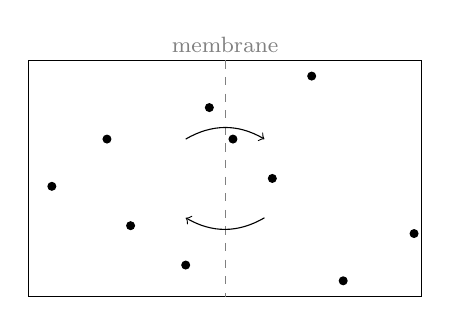
\begin{tikzpicture}
    \draw[draw=black] rectangle ++(5,3);
    \draw[gray,dashed](2.5,3)--(2.5,0);
    \node[circle,draw,fill=black,inner sep=1pt] at (1,2) {};
    \node[circle,draw,fill=black,inner sep=1pt] at (0.3,1.4) {};
    \node[circle,draw,fill=black,inner sep=1pt] at (2.3,2.4) {};
    \node[circle,draw,fill=black,inner sep=1pt] at (2,0.4) {};
    \node[circle,draw,fill=black,inner sep=1pt] at (1.3,0.9) {};

    \node[circle,draw,fill=black,inner sep=1pt] at (2.6,2) {};
    \node[circle,draw,fill=black,inner sep=1pt] at (4,0.2) {};
    \node[circle,draw,fill=black,inner sep=1pt] at (3.1,1.5) {};
    \node[circle,draw,fill=black,inner sep=1pt] at (4.9,0.8) {};
    \node[circle,draw,fill=black,inner sep=1pt] at (3.6,2.8) {};

    \node[gray] at(2.5, 3.2) {\footnotesize membrane};
    \draw [->] (2,2) to [bend left] (3,2);
    \draw [<-] (2,1) to [bend right] (3,1);
\end{tikzpicture}
		\end{figure}
	\end{minipage}\par
	The difference with respect to the previous example is that now the process is a spatially inhomogeneous (but time homogeneuos) RW on $S$ finite. \\
	Define 
	\begin{equation*}
		X^{(N)}(t):= \frac{Y^{(N)}_{\lfloor Nt \rfloor} - N}{\sqrt{N}}
	\end{equation*}
	which implies 
	\begin{equation*}
		Y^{(N)}= i \quad \implies \quad i=x \sqrt{N}+ N
	\end{equation*}
	when $X^{(N)}(t) = x$.\\
	Let's rewrite the probabilities in terms of the $x$:
	\begin{align*}
		p_{x} (\Delta X^{(N)}(t) &= \pm \frac{1}{\sqrt{N}})= \mathbb{P}(\Delta Y^{(N)}_{\lfloor t/h_N \rfloor}= \pm 1| i = x\sqrt{N}+N)   \\
		&= \frac{1}{2} \pm \frac{N - (x \sqrt{N} + N}{2 N} \\
		&= \frac{1}{2} \pm\frac{x}{2 \sqrt{N}}
	\end{align*}
	spatial inhomogeneity. \\
	As we can see, we got a result very similar to the previous one with $x$ in place of $\mu$. \\
	\begin{align*}
		\mathbb{E}(\Delta X^{(N)}(t)) &= \frac{1}{\sqrt{N}}(\frac{1}{2} - \frac{x}{2 \sqrt{N}}) - \frac{1}{\sqrt{N}}(\frac{1}{2} + \frac{x}{2 \sqrt{N}}) \\
		&= - \frac{x}{2N} - \frac{x}{2N} = -\frac{x}{N} \hspace{ 0.5 cm} (h_N = \frac{1}{N};  \ \mu (x) = -x)
	\end{align*}
	\begin{equation*}
		\mE_x[(\Delta X^{(N)}(t))^2] = \frac{1}{N}(\frac{1}{2}-{\cancel{\frac{x}{2\sqrt{N}}}}) + \frac{1}{N}(\frac{1}{2}+{\cancel{\frac{x}{2\sqrt{N}}}}) = \frac{1}{N}
	\end{equation*}
	So, again, $\sigma^2(x) \equiv 1$.
	It is immediate to verify that the moment of order $4$:
	\begin{equation*}
		\mE_x[(\Delta X^{(N)}(t))^4] =O(\frac{1}{N^2})= o (\frac{1}{N})= o (h_N)
	\end{equation*}
	which implies that 
	\begin{equation*}
		X^{(N)} \xrightarrow{d} X
	\end{equation*}
	such that 
	\begin{equation*}
		d X(t) = - X(t) dt + d B(t), \quad X(t) \in \mR
	\end{equation*}
	called \textbf{Ornstein-Uhlenbeck diffusion}, stationary with respect to 
	\begin{equation*}
		N(0,\frac{1}{2})
	\end{equation*}
	It has applications in math finance and in biology. 
	Mean reversion: when it is the positive it pushes back to zero and when it is negative the process is pushed up to return to the $0$ that is the long mean of the process.
	This is particular because is a process that is stationary (BM is not stationary and this property is useful in many application mathfinance, bioology). \\
	We sent by $N$, we rescale and we determine a transformation of the previous one. We plot it and we find its Gaussian distribution. \\
	It can be seen as a continuous-time analogue of AR(1).\\
	Discretize over $\Delta t$ interval to get 
	\begin{equation*}
		\underbracket{\Delta  X_k}_{X_{k+1}-X_{k}} = - X_k \Delta t + \sqrt{\Delta t} \cdot\varepsilon_k 
	\end{equation*}
	where 
	\begin{equation*}
		\varepsilon_k \stackrel{i.i.d}{\sim}
		\mathcal{N}(0,\frac{1}{2})
	\end{equation*}
	which implies that 
	\begin{align*}
		\mE(\Delta X_k) ) & = - X_k \Delta t \\
		\mV ar(\Delta X_k) &= \frac{\Delta t}{2}
	\end{align*}
	and we write
	\begin{equation*}
		X_{k+1} = X_k -X_k \Delta t + \sqrt{\Delta t}\epsilon_k=\underbrace{1-\Delta t}_{a}X_k + \underbrace{\sqrt{\Delta t}}_{b}\epsilon_k
	\end{equation*}
	\item \textbf{Branching Processes}
	Consider 
	\begin{equation*}
		Y^{(N)}_n \text{ a BP   } Y^{(N)}_n = \sum_{i=1}^{Y^{(N)}_{n-1}} Z_i^{(N)}
	\end{equation*}
	where $n$ refers to the step, while $N$ the parameterisation and \\
	$Z_i^{(N)} \stackrel{i.i.d.}{\sim}$  
	with mean $\mu^{(N)} \in \mR$ and variance $\sigma^2 > 0$. 
	\begin{equation*}
		\mE[Y_n^{(N)}|Y_{n-1}^{(N)}=y] = \mu^{(N)}y  \hspace{0.5 cm}\implies \mE_y[\Delta Y_n^{(N)}]= \mu^{(N)} y -y =y(\mu^{(N)}-1)
	\end{equation*}
	Now observe:
	\begin{equation*}
		\text{Var}_y(Y_n^{(N)})=\sigma^2 y
	\end{equation*}
	Define
	\begin{equation*}
		X^{(N)}:= \frac{Y^{(N)_{\lfloor Nt \rfloor}}}{N}    
	\end{equation*}
	which implies that 
	\begin{equation*}
		X^{(N)}(t) = x \implies y = N x
	\end{equation*}
	\begin{equation*}
		\mE_x[\Delta X^{(N)}(t)]=\frac{1}{N}\mE_y[\Delta Y^{(N)}_{\lfloor Nt \rfloor}]=\frac{1}{N}y(\mu^{(N)}-1)
	\end{equation*}
	\begin{align*}
		\mE_x [(\Delta X^{(N)}(t))^2] &= \var_x (\Delta X^{(N)}(t)) + (\mE_x[\Delta X^{(N)}(t)])^2 \\
		& = \frac{1}{N^2} \underbrace{\var_y (\Delta Y_n )}_{\var_y (Y_{n+1} )+0 } + \frac{1}{N^2} Y^2(\mu^{(N)}-1)^2 \\
		&= \frac{1}{N^2}\sigma^2 y + \frac{1}{N^2}y^2(\mu^{(N)}-1)^2 
	\end{align*}
	if we let $\mu^{(N)}$ be a perturbation of 1, i.e. $\mu^{(N)}= 1 \frac{m}{N}$ so that $\mu^{(N)}- 1=  \frac{m}{N}$, then
	\begin{equation*}
		\mE_x [\Delta X] = \frac{1}{N} y \frac{m}{N} = \frac{my}{N^2} = \frac{mx}{N}
	\end{equation*}
	since $y = Nx$
	\begin{equation*}
		\mE_x[(\Delta X)^2] = \frac{\sigma^2 x }{N} + \underbrace{\frac{1}{N^2} N^2 x^2 \frac{m^2}{N^2}}_{o(\frac{1}{N})}
	\end{equation*}
	$h_N= \frac{1}{N}$, $\mu (x)= mx $ and $\sigma^2 = x$. \\
	\begin{equation*}
		\implies \qquad X^{(N)} \xrightarrow{d} X \qquad \text{s.t.}
	\end{equation*}
	such that 
	\begin{equation*}
		d X(t) = m X(t) dt + \sigma \sqrt{X(t)} dB(t)
	\end{equation*}
	This process is called 
	\begin{itemize}
		\item \textbf{Cox-Ingersoll-Ross diffusion} in math finance
		\item \textbf{Continuous state Branching Process} in math biology
	\end{itemize} 
	So, if we touch $0$ we are going to stay there forever. This is the situation we gained talking about Markov Chains and extinction of a certain population: once reached, the population stays extinguished. \\
	$0$ is an \textit{absorbing state}. \\
	This reasoning has also a discretised counterpart. \\
	\item \textbf{Wright-Fisher processes}\\
	The transitions
	\begin{equation*}
		Y_{n+1}^{(N)}|Y_n=i \sim \text{Binom}(N,\frac{i}{N})
	\end{equation*}
	are space inhomogeneous and indexed by $N$.
	
	\begin{equation*}
		X^{(N)}(t) := \frac{Y^{(N)}_{\lfloor Nt\rfloor}}{N}
	\end{equation*}
	the percentage of type $0$. \\
	For brevity of notation, 
	\begin{equation*}
		Z_x := (X^{(N)}(t+\frac{1}{N})|X^{(N)}(t)=\underbrace{x}_{i/N})\sim\frac{1}{N}\text{Binom}(N,x)
	\end{equation*}
	Let's now comput the first two moments, starting with the first one:
	\begin{equation*}
		\mE_x[\Delta X^{(N)}(t)] = \mE(Zx) - x  =\frac{1}{N} N x = 0
	\end{equation*}
	and moving on to the second moment:
	\begin{align*}
		\mE_x[(\Delta X^{(N)}(t)^2] &= \text{Var}_x[\underbracket{\Delta X(t)}_{z_x-x}] + (\underbrace{\mE_x[\Delta X(t)]}_{0})^2 \\
		&= \frac{1}{N^2}Nx(1-x) = \underbrace{\frac{1}{N}}_{h_N} \underbrace{x(1-x)}_{\sigma^2 (x)}
	\end{align*}
	So 
	\begin{equation*}
		X^{(N)}\xrightarrow{d} X
	\end{equation*}
	such that 
	\begin{equation*}
		dX(t) = \sqrt{X(t) (1-X(t))} d B(t)
	\end{equation*}
	\begin{figure}
		\centering
		
\pgfmathsetseed{654}
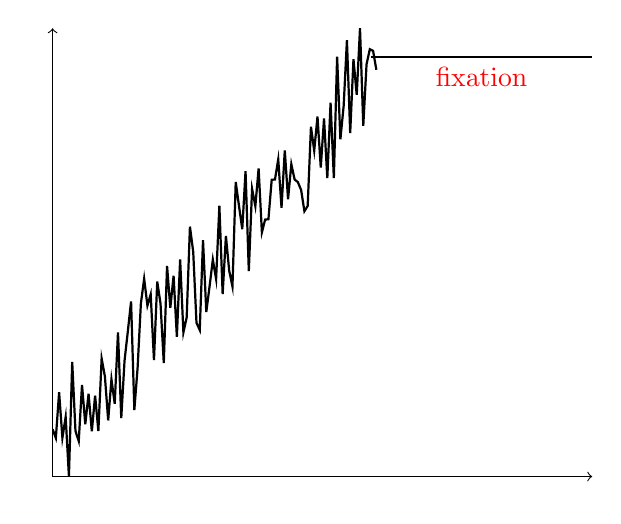
\begin{tikzpicture}
\begin{axis}[
                xlabel=\empty,
                x axis line style={->,opacity=100},
                ylabel=\empty,
                axis y line=left,
                %ymin=-0.6,ymax=2,
                xmin=0,xmax=50,
                y axis line style={->,opacity=100},
                ytick=\empty,
                xtick={85,170},
                xticklabels={$t_1$,$t_2$},
                axis x line*=bottom
                   ]     
    \addplot[black,domain = 0:30,
        samples = 100,
        thick] {2*x+10*rand};
    \addplot[black,thick]coordinates{(29.5,61.5)(50,61.5)}node[red,midway,below]{fixation};
\end{axis} %fashion
\end{tikzpicture}
	\end{figure}
	If all offspring are of type $0$, we are going to have always type $1$. Here it is the same way of thinking. \\
	Add mutations:
	\begin{equation*}
		Y_{n+1}| Y_n =i \sim Binom(N,p_i)
	\end{equation*}
	where $p_i = \alpha(1- \frac{i}{N}) + (1-\beta )\frac{i}{N}$ and, in turn, 
	\begin{align*}
		\alpha &= \mathbb{P}(1 \rightarrow 0) \\
		\beta &= \mP(0 \rightarrow 1)
	\end{align*}
	\begin{equation*}
		\Tilde{Z}_x := (X^{(N)}(t+\frac{1}{N})|X^{N}(t) = x) \sim \frac{1}{N} Binom(N, p_x)
	\end{equation*}
	where $x= \frac{i}{N}$ and $p_x = \alpha(\-x) + (1-\beta )x$. \\
	If we compute the increment of $X$, we have
	\[
	\mE_x[\Delta X(t)] = \mE_x[\Tilde{Z}_x] = x = \frac{1}{N} N p_x - x = \ldots = \frac{1}{N} \underbrace{[\alpha (1-x)-\beta x]}_{\mu(x)}
	\]
	
	% is there 2 in the [ ] at the end where it is underbraced?
	\begin{exercise}
	As exercise, show that 
	\begin{equation*}
		\mE_x[(\Delta X(t))^2]= \dots = \frac{1}{N}
		\underbrace{x(1-x)}_{\sigma^2(x)} + o (\frac{1}{N})
	\end{equation*}
	which implies that 
	\begin{equation*}
		X^{(N)} \xrightarrow{d} X
	\end{equation*}
	such that 
	\begin{equation*}
		d X(t) = [2(1-X(t)) - \beta X(t)]dt + \sqrt{ X(t) (1-X(t))} dB(t) = 0
	\end{equation*}
\end{exercise}
	if $X(t) = 0,1$. 
	\begin{itemize}
		\item at $X(t)=0$ we have $dX(t)= \alpha dt$
		\item at $X(t)=1$ we have $dX(t)= -\beta dt$
	\end{itemize}
	\begin{figure}[H]
		\centering
		
\pgfmathsetseed{654}
\begin{tikzpicture}
\begin{axis}[
                xlabel=\empty,
                x axis line style={-,opacity=100},
                ylabel=\empty,
                axis y line=left,
                ymin=-0,ymax=60,
                %xmin=0,xmax=50,
                y axis line style={-,opacity=0},
                ytick=\empty,
                xtick=\empty,
                %axis x line=bottom top
                   ]     
    \addplot[black,domain = 0:30,
        samples = 100,
        thick] {2*x+10*rand};
        \addplot[black,domain = 30:80,
        samples = 100,
        thick] {-1.5*x+10*rand+90};
        \addplot[black,domain = 80:240,
        samples = 250,
        thick,xshift={-20pt}] {1.4*(x+200)+10*rand-400};
        \draw [-{Stealth},very thick,red] (35,60) to (35,50);
        \draw [-{Stealth},very thick,red] (80,00) to (80,10);
\end{axis} %fashion
\node[] at (-0.5,5.7){1};
\node[] at (-0.5,0){0};
\end{tikzpicture}
	\end{figure}
	An application of the scaling limits is suggested by what we just wrote (?).\\
	\begin{itemize}
		\item we can avoid the computation of the conditional probability, which is very tricky.
		\item if the variance is small we cannot conclude that much. If it is too big, the process moves too much. So we study the limit diffusions under the problematic of rescaling. 
	\end{itemize}
	\end{enumerate}
	\begin{figure}[H]
		\centering
		\includegraphics[width=0.7\linewidth]{../drawings/samplepaths.png}
	\end{figure}
	\includepdf[pages=10,pagecommand={}]{../drawings/Lec 16.pdf}
	A possible application of these concepts is in the approximation of stationary distributions:\par
	\begin{minipage}{0.5\textwidth}
		\includegraphics[width=1\linewidth]{../drawings/approxstation.png}
	\end{minipage}\hfill
	\begin{minipage}{0.5\textwidth}
		\includegraphics[width=1\linewidth]{../drawings/approx2.png}
	\end{minipage}
	Another application may be the tuning of the variance in a Random Walk Metropolis-Hastings algorithm (trough the "Goldilocks" method) using scaling limits.
	\begin{figure}[H]
		\centering
		\includegraphics[width=0.67\linewidth]{../drawings/goldilocks.png}
	\end{figure}
	We can also study different rescalings of a class of Random Walk Metropolis-Hastings algorithms and how to tune the variance of the proposal distribution accordingly:
	\begin{figure}[H]
		\centering
		\includegraphics[width=1\linewidth]{../drawings/variousrescalings.png}
	\end{figure}
\end{document}